\chapter{Integrating with the OpenPRA Web Platform}

% Use the openpra web app paper.
% - Bring the technical elements discussions (Front-end perspective)
% - Bring the OpenPRA-\acrshort{mef} \acrshort{json} schema developed by Rahul 
% - Describe the concrete \acrshort{rest} \acrfull{api}s, along with screenshots from Swagger)
% - Distinguish the v2 app (developed during this study) from the v1.
% - Address gaps and limitations (there are many!).
% - Bring the screenshots from webapp/paper.

\section{OpenPRA Web-App Architecture}
The system consists of a web‑based front end, a standardized OpenPRA \acrfull{mef} schema, a back end providing \acrfull{rest}ful \acrfull{api}s, distributed databases, and a distributed job queue, as shown in figure \ref{fig:openpra_overview}. Each layer has a distinct role:

\begin{figure}[h!]
  \centering
  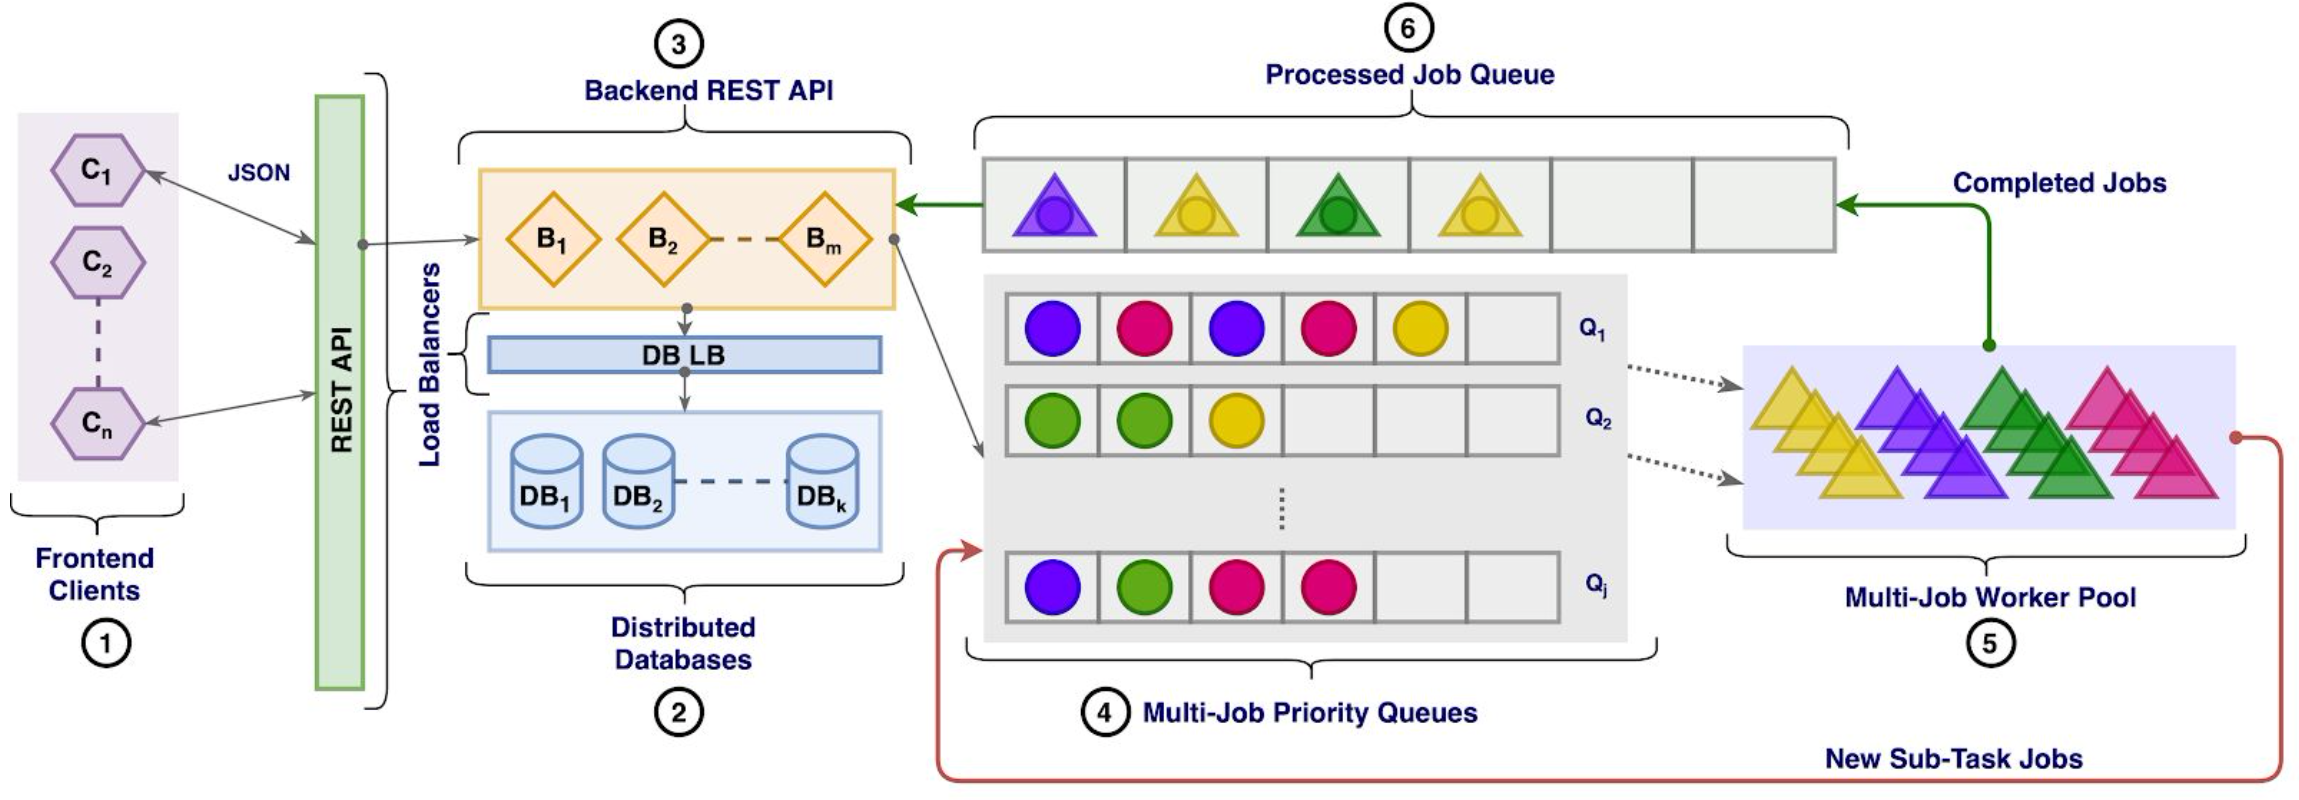
\includegraphics[width=0.9\textwidth]{4_proposed_solution/web_app/figures/openpra_overview.png}
  \caption{High-level functional overview of the framework.}
  \label{fig:openpra_overview}
\end{figure}

\begin{itemize}
\item \textbf{Front-end (Web \acrshort{ui})}: Provides a user interface for editing \acrshort{pra} models, configuring solver parameters and for visualizing analysis results. Figure \ref{fig:landing_page} shows the landing page of the web app.
\item \textbf{OpenPRA \acrshort{mef} schemas}: Defines a common \acrshort{json} model-exchange format that validates the \acrshort{pra} model data. These schemas ensure that all models follow a consistent structure across the platform.
\item \textbf{Backend (\acrshort{rest} \acrfull{api}s)}: Acts as the coordination layer. It exposes endpoints for managing \acrshort{pra} models, triggers computations, and orchestrates interactions with the database.
\item \textbf{Distributed databases}: A \acrfull{nosql} database cluster that stores projects, \acrshort{pra} model related metadata and analysis results.
\end{itemize}

Data flows through these layers as users interact with the system. In a typical workflow:
\begin{enumerate}
\item The user constructs or updates a \acrshort{pra} model in the front-end, generating structured \acrshort{json} data conforming to the OpenPRA \acrshort{mef} schema.
\item The front-end sends this data to the backend via a \acrshort{rest} \acrshort{api} call; the backend validates the input and, if the request is to save or modify a model, persists the data in the distributed databases.
\item If the user requests a quantitative analysis, the backend publishes the request as a job to the distributed queuing system with references to the stored model and solver parameters.
\item A worker retrieves the job from the queue, performs the calculation using the user defined solver, and writes the results back to the database.
\item The backend then makes the computed results available via its \acrshort{api}, and the front-end fetches them to complete the workflow.
\end{enumerate}

\section{User Interface}

\subsection{Web-Based Front-end}

The web-based front-end of OpenPRA is designed to address the existing gaps in the current ecosystem of \acrshort{pra} tools. The front-end tries to meet a comprehensive set of requirements demanded by evolving technological landscape, including:

\begin{itemize}
\item \textbf{User friendly interface:} Provides an intuitive, browser-based \acrshort{ui} with built-in visualization tools, lowering the barrier for users of all technical backgrounds.
\item \textbf{Web based access:} Allows secure access via \acrshort{https} without client installation, supporting remote workflows.
\item \textbf{Open source platform:} Freely available and community‑driven, promoting transparency, collaboration, and continuous improvement.
\item \textbf{Collaborative environment:} Enables multiple users to work concurrently on the same \acrshort{pra} model, improving teamwork and efficiency across multiple teams.
\item \textbf{Version control:} Records changes to a model, persists revision history, and supports version rollback whenever a prior state must be restored.  
\item \textbf{Support for a wide range of risk models:} Provides editors for event trees, fault trees, Markov chains, Bayesian networks, and other formalisms, enabling analysts to choose a risk model that best represents their system.  
\item \textbf{Choice of quantification engines:} Integrates multiple built‑in and third‑party solvers so analysts can select an algorithm most suitable for their use case.  
\item \textbf{Interoperability:} Serializes models to the standardized OpenPRA \acrshort{mef} \acrshort{json} format, ensuring seamless data exchange with external tools and workflows.
\item \textbf{Customizability:} Allows users to tailor the interface, workflows, and analysis parameters to their specific project requirements.
\end{itemize}

\begin{figure}[h!]
  \centering
  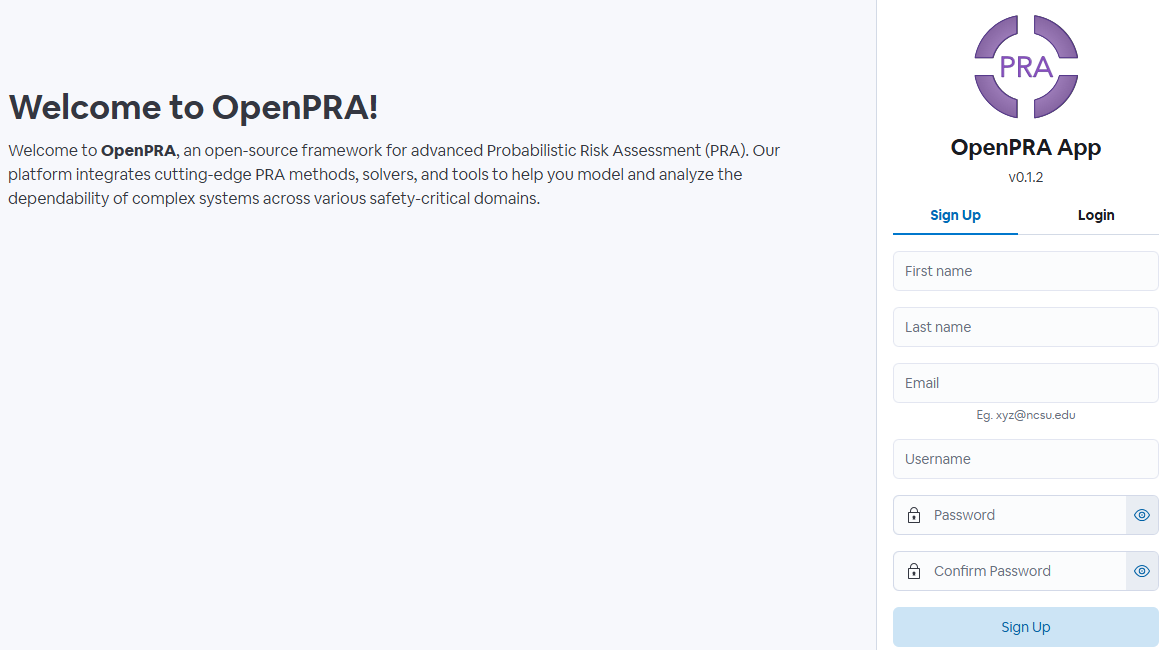
\includegraphics[width=0.9\textwidth]{4_proposed_solution/web_app/figures/landing_page.png}
  \caption{Landing page of the OpenPRA web application.}
  \label{fig:landing_page}
\end{figure}

\subsection{Analysis Modes, Types and Risk Models}

The front-end supports a wide range of analysis modes, analysis types and risk models. This enables users to tailor their risk assessment process to their specific needs and preferences. An overview of the supported analysis modes have been given below. Figures \ref{fig:analysis_modes_types} and \ref{fig:data_analysis} show overviews of internal event and data analyses.

\begin{itemize}
  \item \textbf{Internal events analysis:} Helps to model events originating within the system such as equipment failures or operator errors, to assess their impact on overall reliability and safety of the system.
  \item \textbf{Internal hazards analysis:} Provides tools to model hazards arising inside the system e.g., fires or floods, and evaluates their potential risk to system integrity.
  \item \textbf{External hazards analysis:} Supports the modeling of external events such as earthquakes, to determine their effects on system performance and safety.
  \item \textbf{Full scope \acrshort{pra} analysis:} Offers a comprehensive analysis of all potential risks, integrating modeling of both internal and external events and hazards.
  \item \textbf{Data analysis:} Enables importing, processing, and analyzing system data such as failure and operational records, using parametric distributions (e.g., from \acrshort{nrc} industry average parameter estimates database) to gain insights into system performance and reliability.
\end{itemize}

Aside from data analysis, each of the listed analysis modes supports the analysis types:

\begin{itemize}
  \item \textbf{Plant operating states analysis:} Analyzes system performance and reliability across different plant modes such as full power, low power, and shutdown to identify plant-state specific risk profiles.
  \item \textbf{Initiating events analysis:} Models and assesses internal or external triggers like equipment failures, human errors, and natural disasters to evaluate their potential to initiate accident sequences.
  \item \textbf{Event sequence analysis:} Analyzes the chain of events following an initiating event to evaluate possible failure pathways and their associated probabilities.
  \item \textbf{Success criteria development:} Defines metrics for successful system operation and assesses the likelihood of meeting these criteria under various operating conditions and event scenarios.
  \item \textbf{System analysis:} Uses modeling techniques such as fault tree analysis and reliability block diagrams to evaluate overall system performance under failure and hazard conditions.
  \item \textbf{Human reliability analysis:} Assesses the impact of active and latent human errors on system safety using an \acrshort{hra} methodology extended from Phoenix.
  \item \textbf{Mechanistic source term analysis:} Models and assesses the release mechanisms of hazardous materials during an accident to determine source terms.
  \item \textbf{Radiological consequence analysis:} Models dispersion and assesses exposure of radioactive materials post‑accident to quantify potential radiological impacts on workers and the public.
  \item \textbf{Uncertainty analysis:} Applies parametric, non‑parametric, and Monte Carlo sampling methods to assess uncertainties in risk assessment inputs and outputs.
  \item \textbf{Risk integration analysis:} Integrates results from individual analyses and models overall system risk as frequency‑consequence curves for a comprehensive risk profile.
\end{itemize}

\begin{figure}
  \centering
  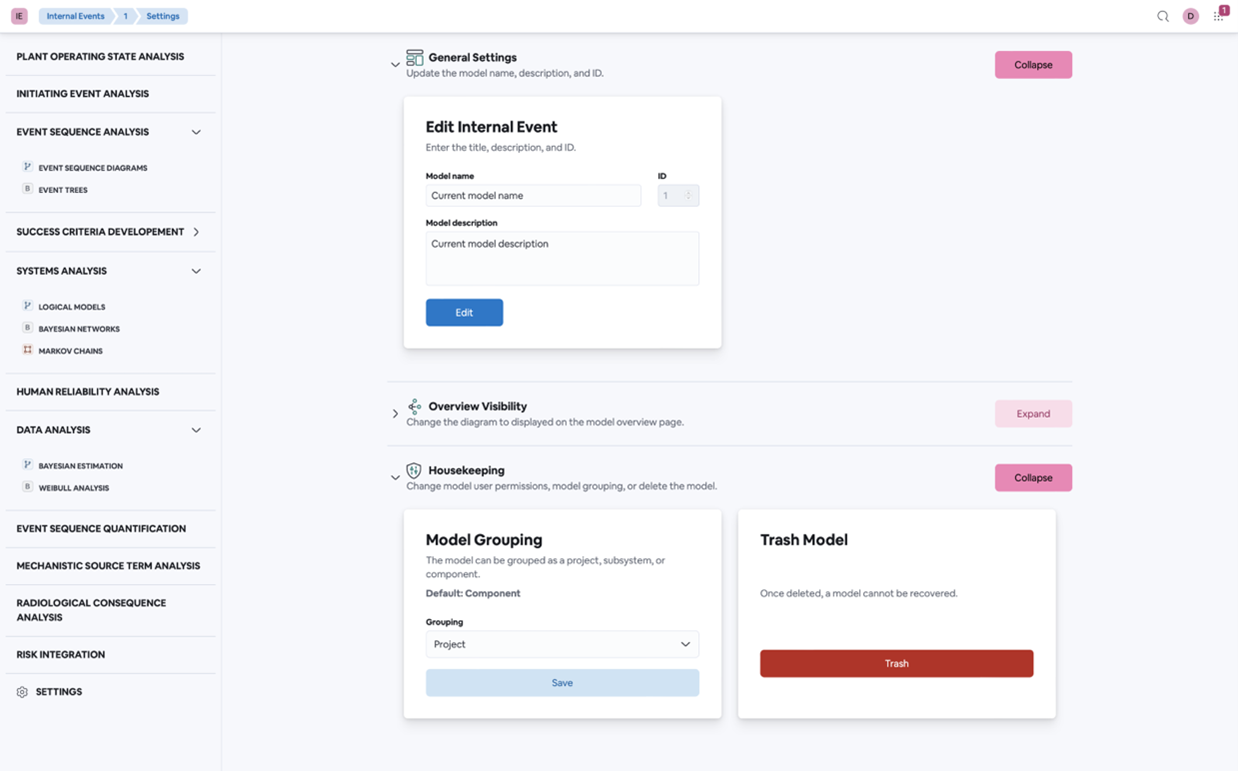
\includegraphics[width=1.0\textwidth]{4_proposed_solution/web_app/figures/analysis_modes_types.png}
  \caption{Internal events analysis overview.}
  \label{fig:analysis_modes_types}
\end{figure}

\begin{figure}
  \centering
  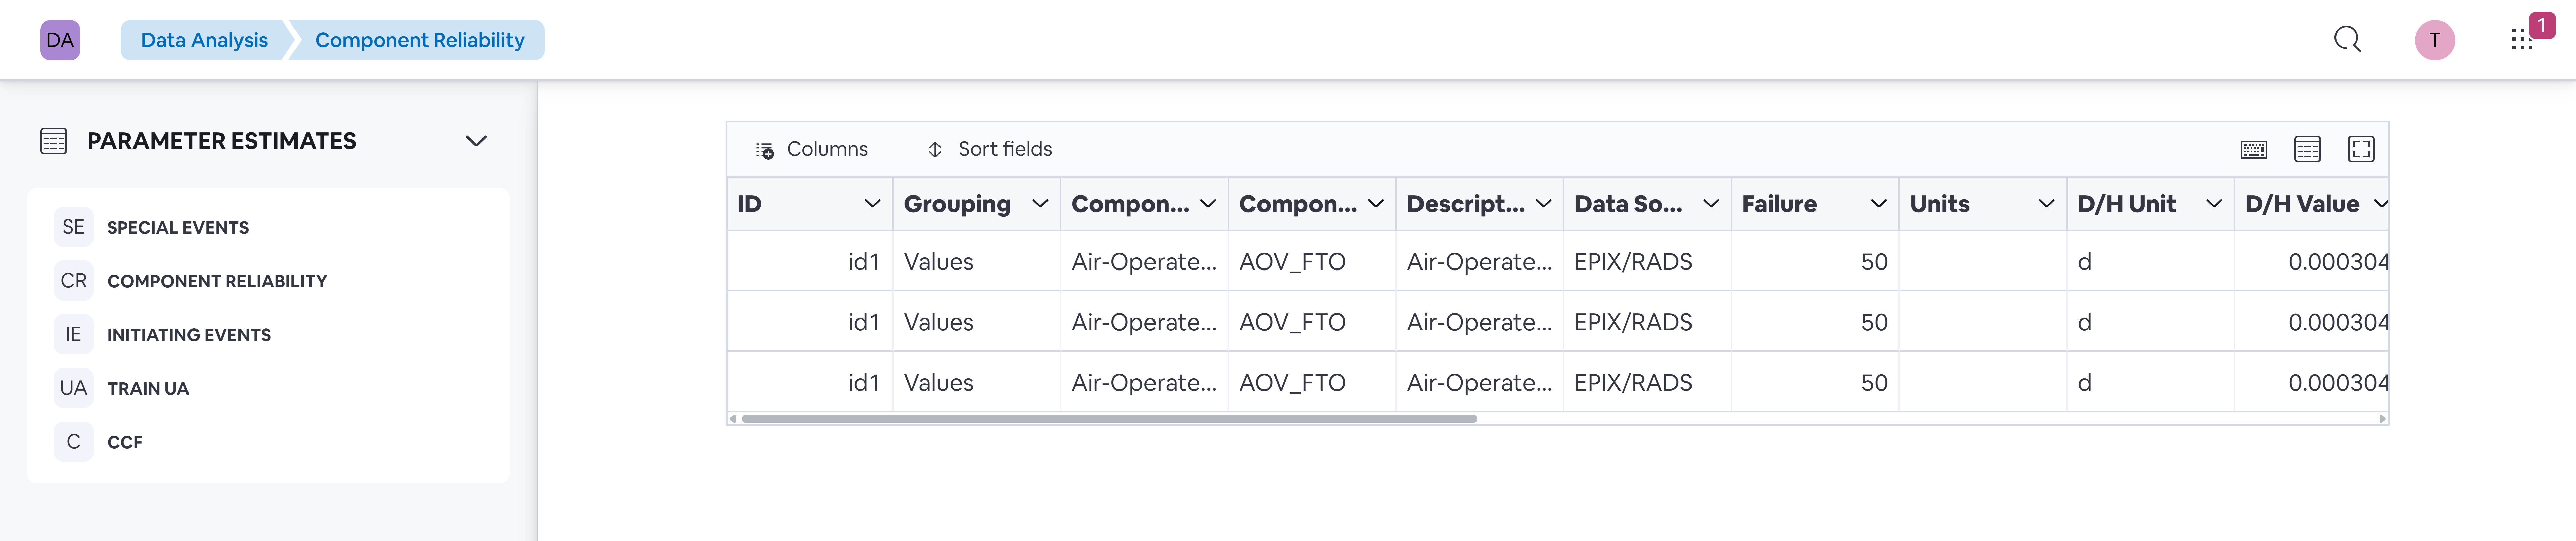
\includegraphics[width=1.0\textwidth]{4_proposed_solution/web_app/figures/data_analysis.png}
  \caption{Data analysis overview.}
  \label{fig:data_analysis}
\end{figure}

The front-end supports a wide array of risk models, each designed to address specific components of the analysis types outlined earlier. Figure \ref{fig:risk_models} shows such four risk models. 

\begin{itemize}
  \item \textbf{Initiating events:} Models and assesses potential triggers using master logic diagrams, \acrshort{fmea}, and heat balance fault trees for internal or external failures (e.g., equipment failures, human errors, natural disasters) that can shift the system into accident sequences.
  \item \textbf{Event sequence diagrams:} Provides compressed‑notation diagrams with support for cycles to model and analyze complex, temporally arranged phenomena following an initiating event.
  \item \textbf{Event trees:} Uses node and branch based diagrams to model and analyze possible sequences of events leading to specific outcomes, assessing the likelihood and consequences of each pathway.
  \item \textbf{Fault trees:} Employs Boolean gate and basic event based diagrams to model combinations of component failures and analyze their contributions to overall system failure.
  \item \textbf{Markov chains:} Applies probabilistic state transition models to analyze system reliability and availability over time through discrete states and transitions.
  \item \textbf{Bayesian networks:} Constructs directed graph models of probabilistic dependencies to analyze uncertain variables and their interactions within complex systems.
  \item \textbf{Probabilistic model checkers:} Integrates dual‑graph error propagation models to model and analyze the propagation of faults, errors, and failures through a cyber‑physical system.
  \item \textbf{Consequence models:} Links end states of event sequences with categorized outcomes (e.g., radiological doses, financial losses) and integrates them into frequency‑consequence curves for comprehensive risk evaluation.
\end{itemize}

%--------------------------------------------------------------
\begin{figure}
  \centering
  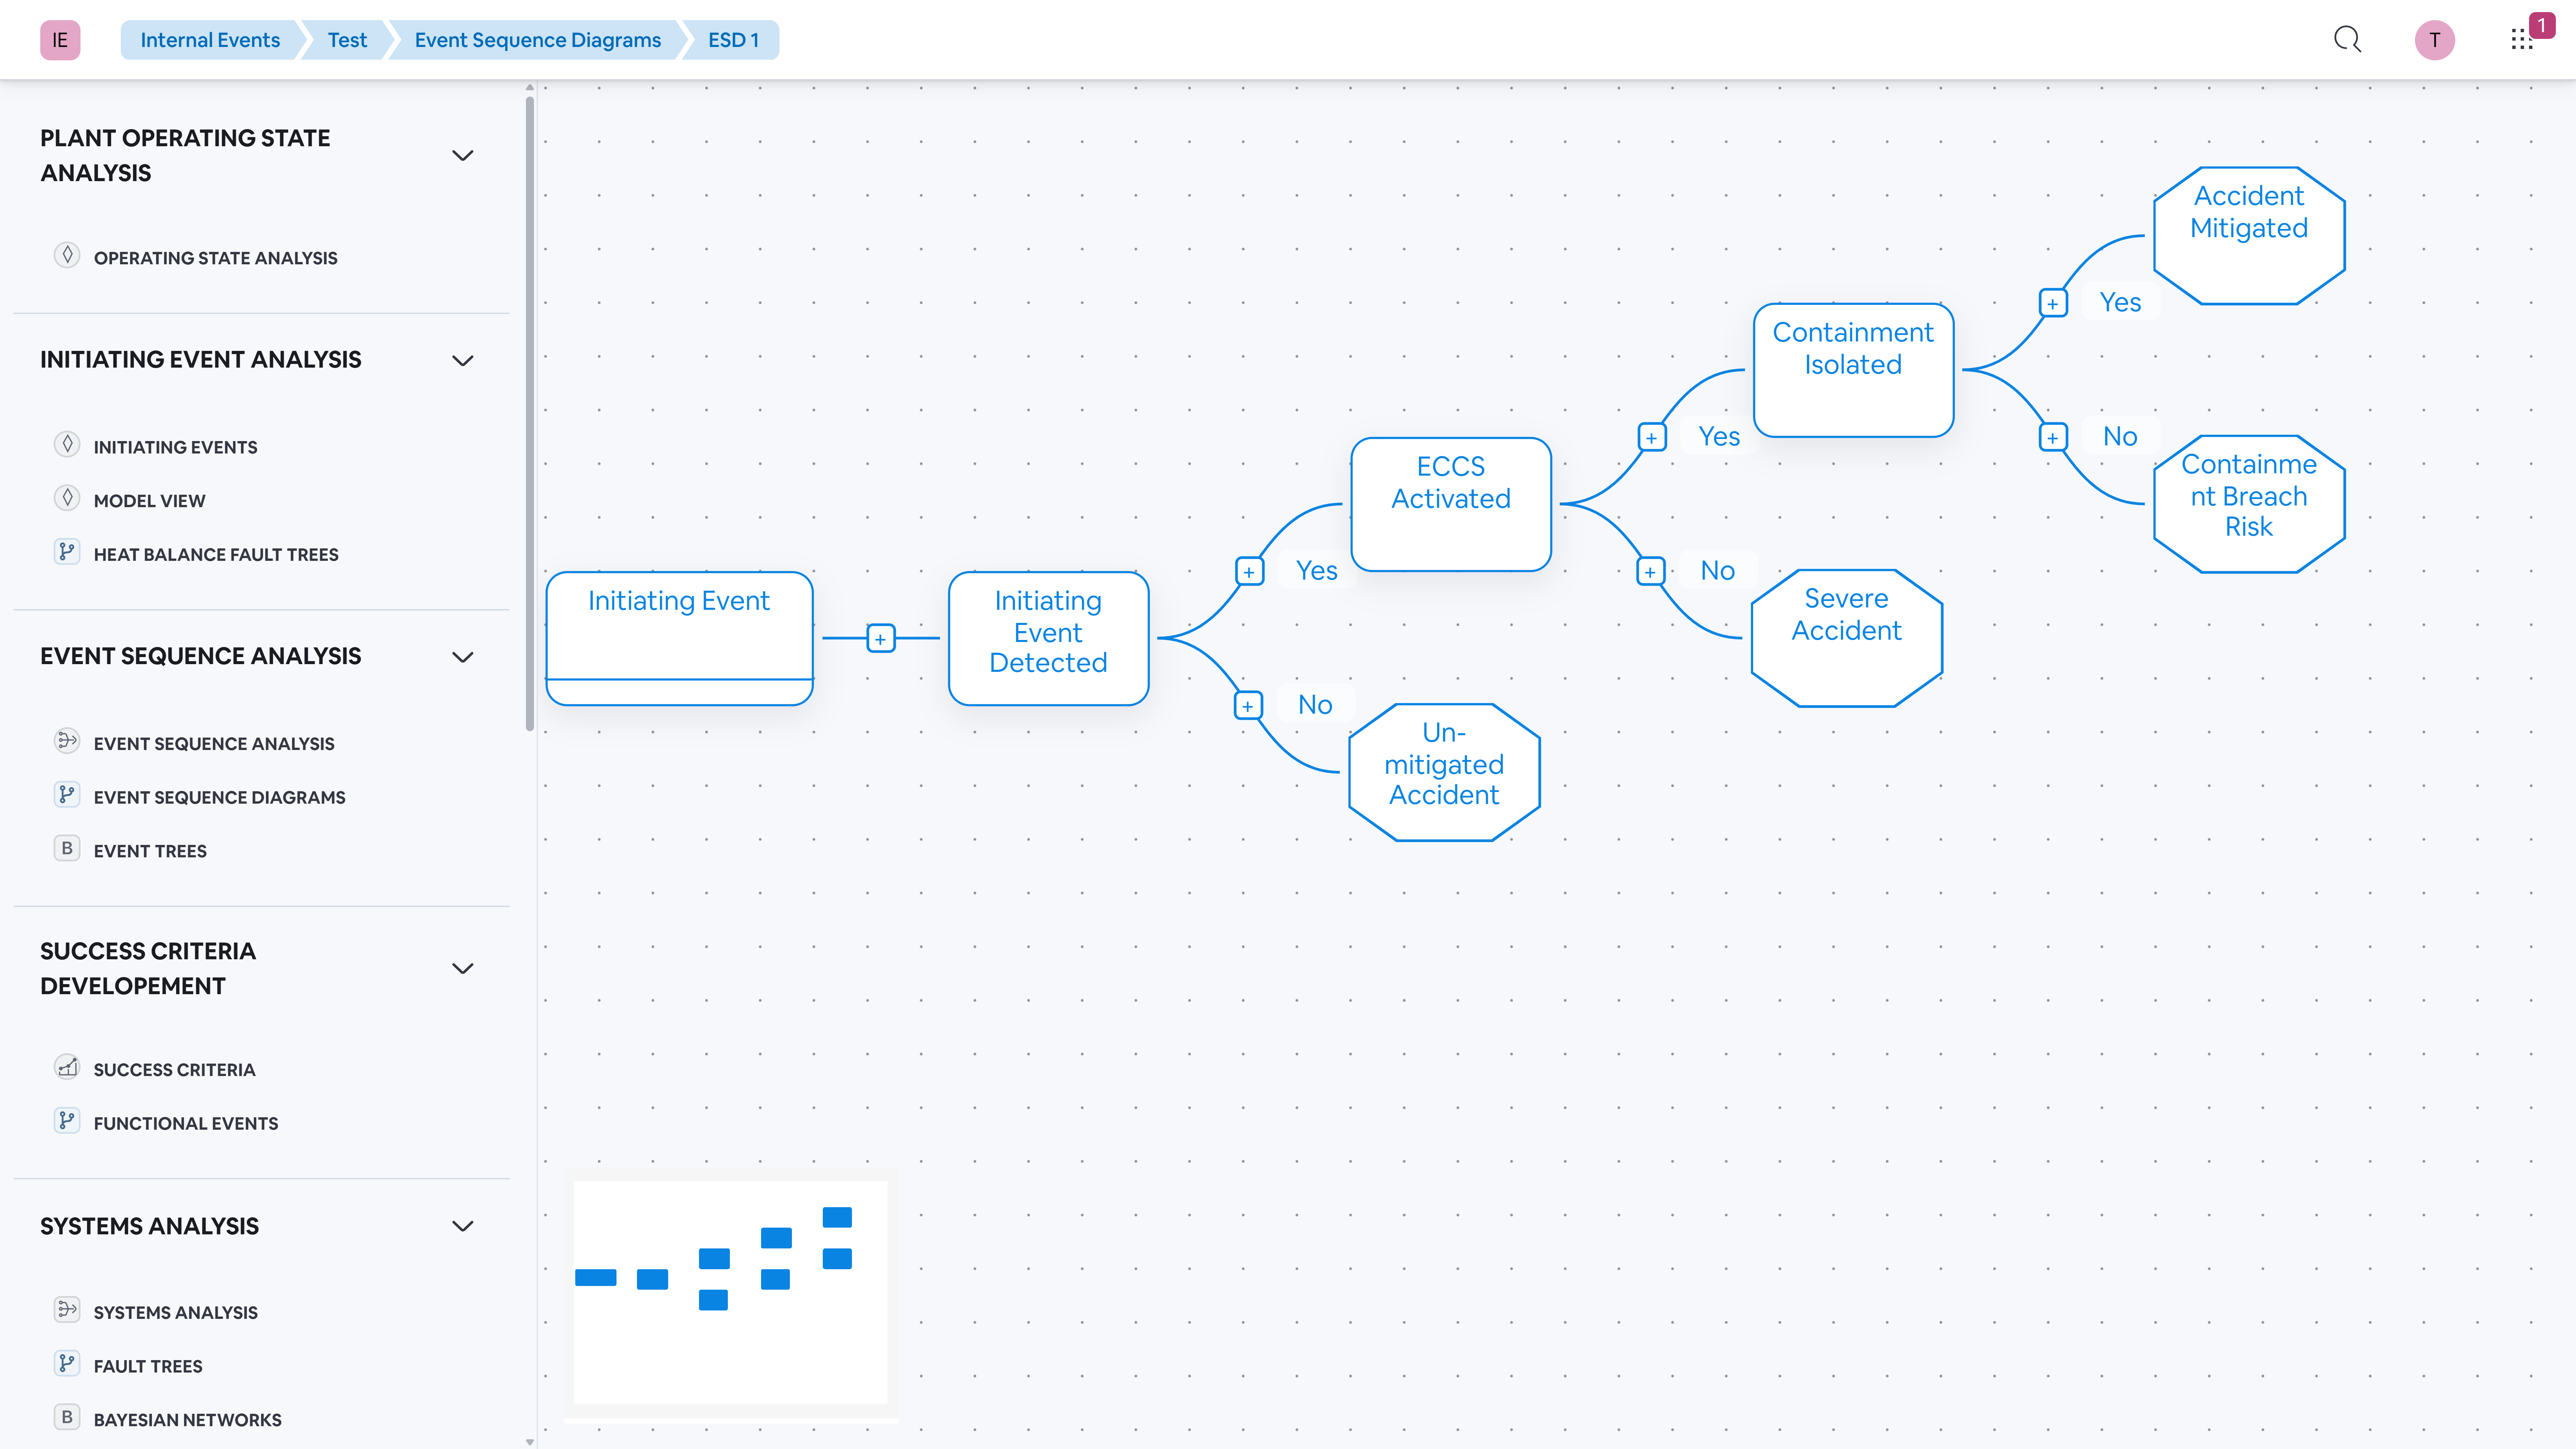
\includegraphics[width=\textwidth]{4_proposed_solution/web_app/figures/esd.png}
  \caption{Event sequence diagram editor.}
  \label{fig:esd_editor}
\end{figure}

%--------------------------------------------------------------
\begin{figure}
  \centering
  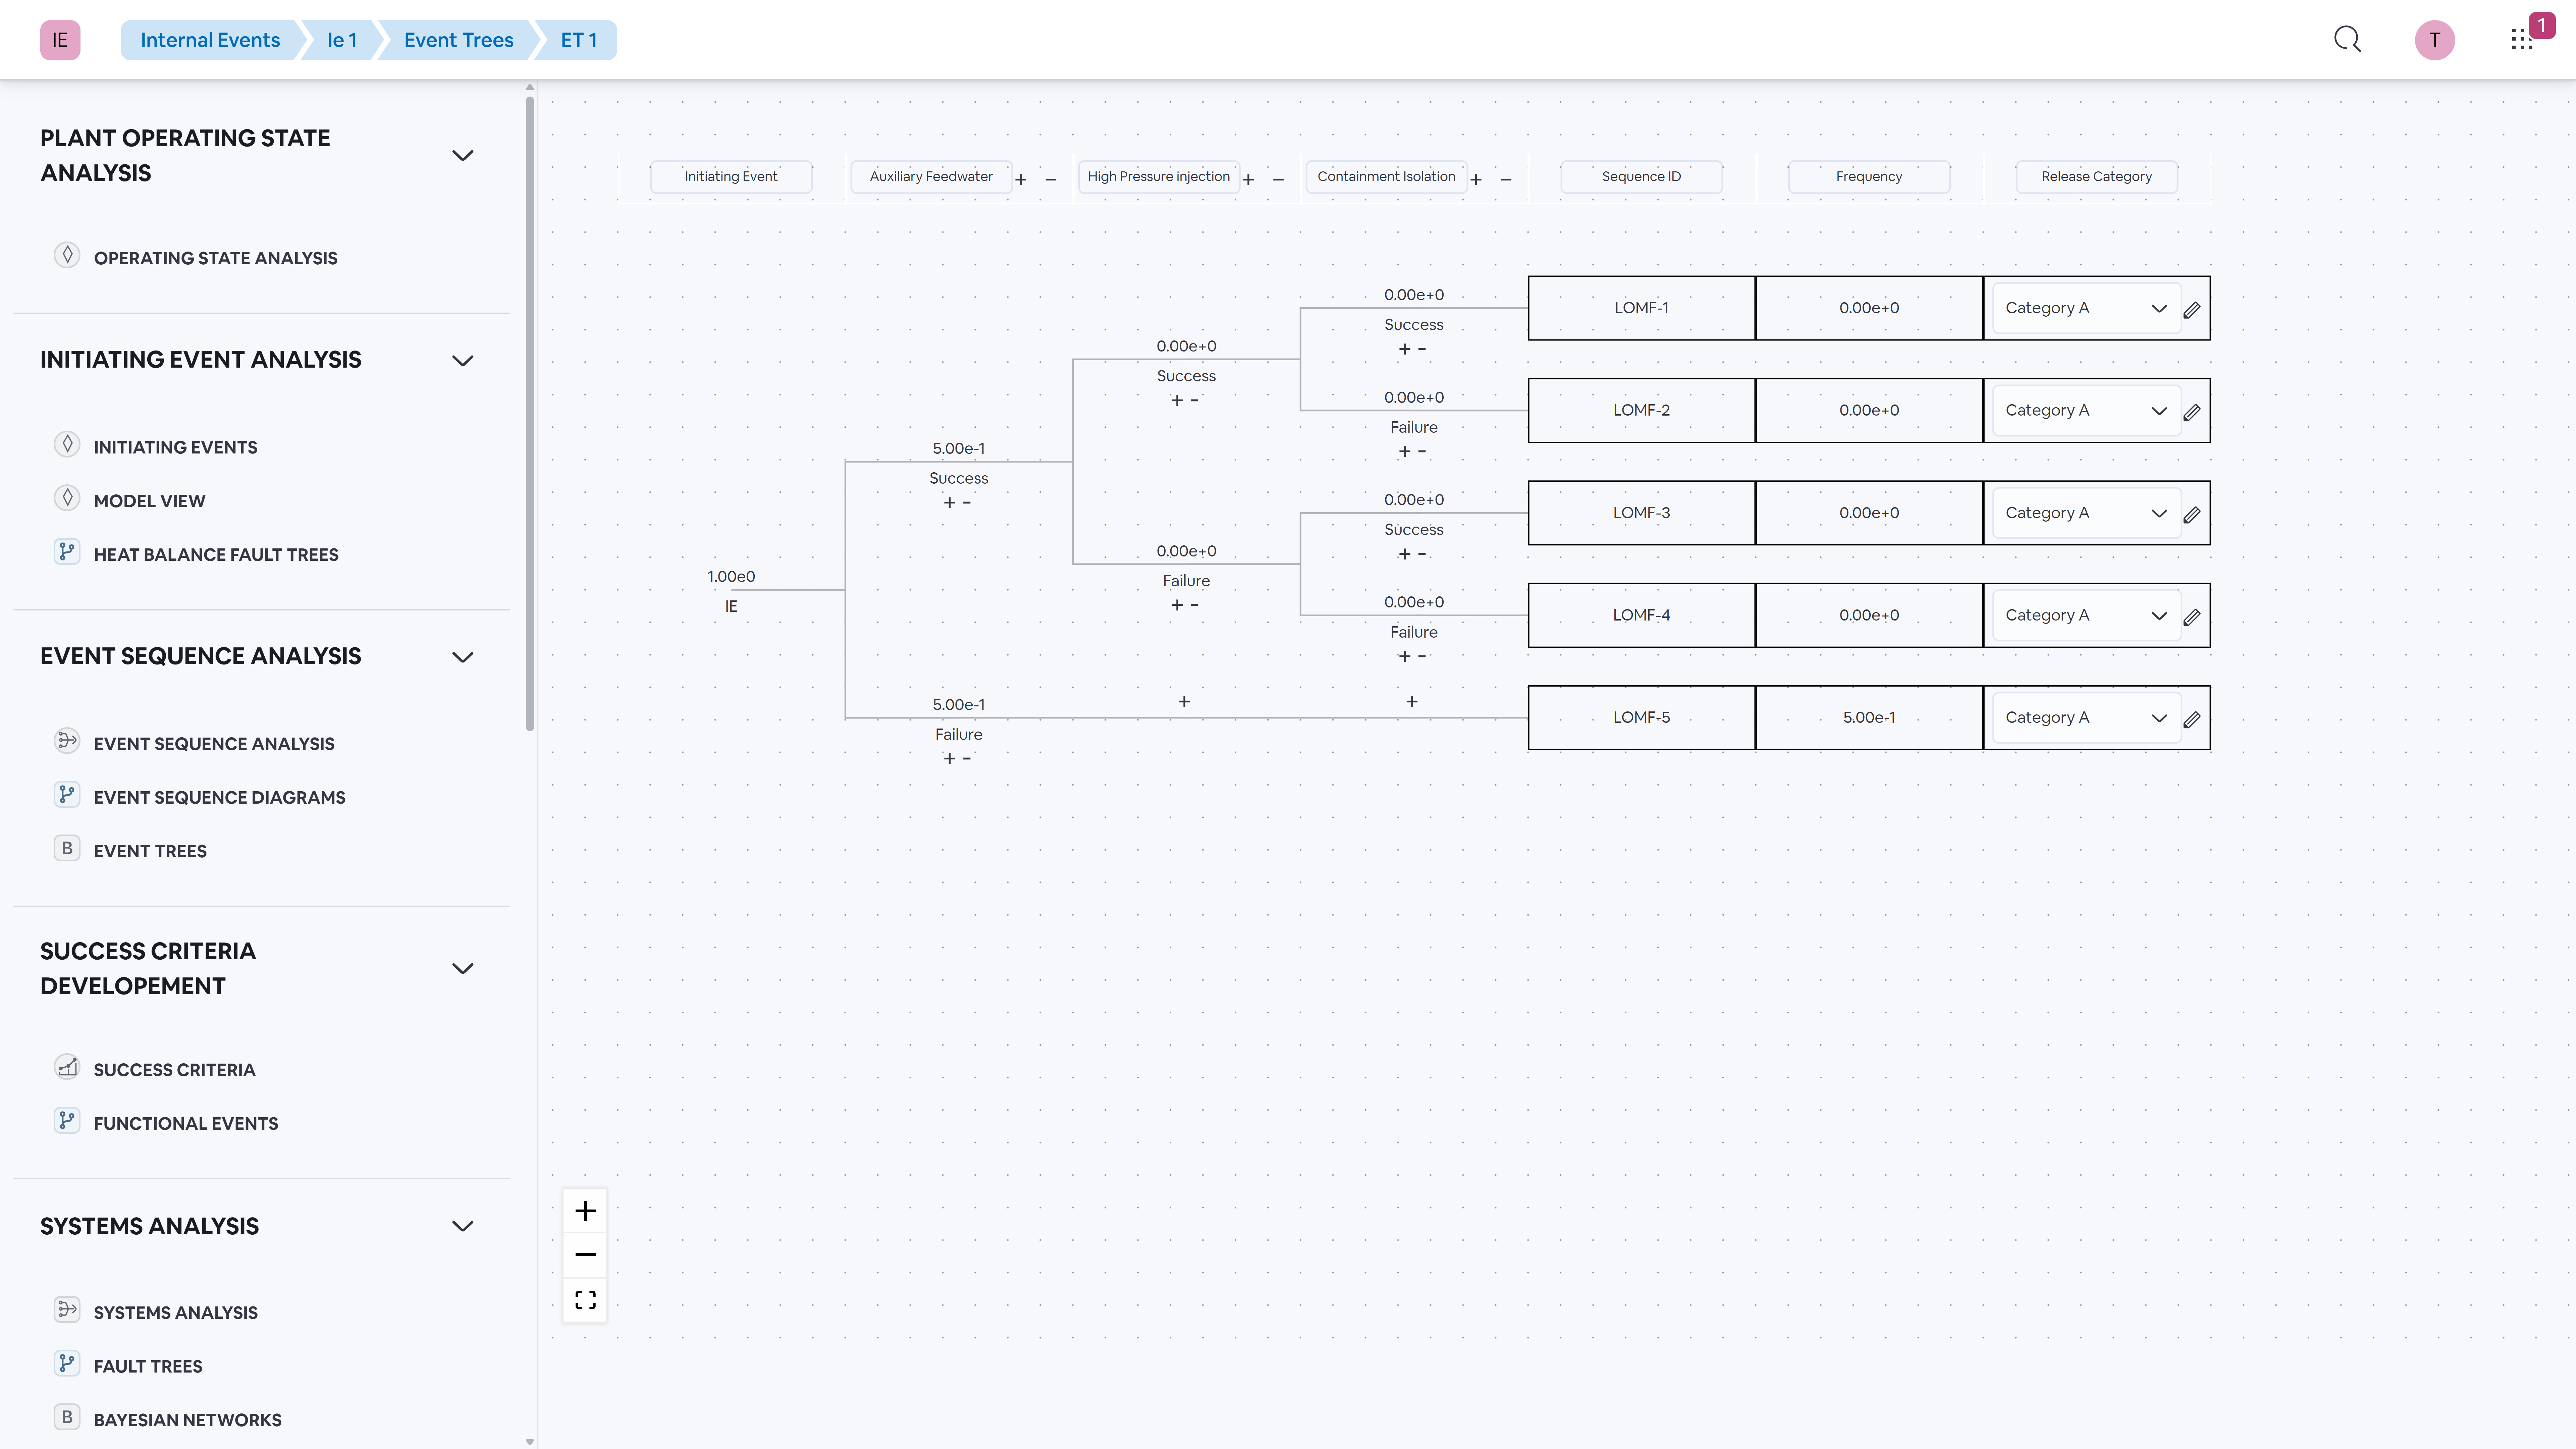
\includegraphics[width=\textwidth]{4_proposed_solution/web_app/figures/et.png}
  \caption{Event tree editor.}
  \label{fig:et_editor}
\end{figure}

%--------------------------------------------------------------
\begin{figure}
  \centering
  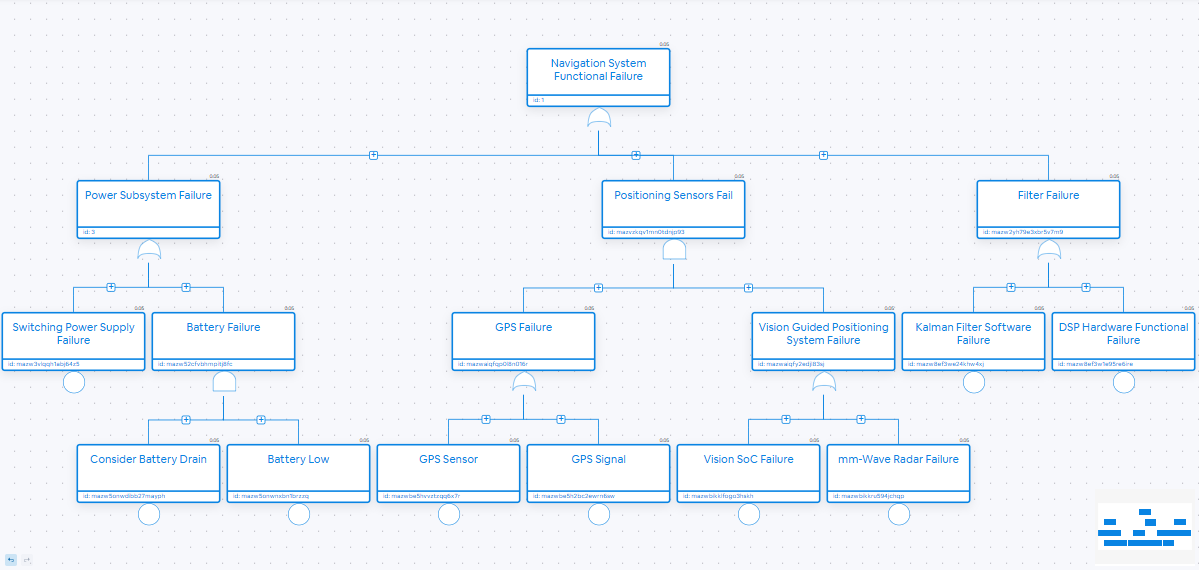
\includegraphics[width=\textwidth]{4_proposed_solution/web_app/figures/ft.png}
  \caption{Fault tree editor.}
  \label{fig:ft_editor}
\end{figure}

%--------------------------------------------------------------
\begin{figure}
  \centering
  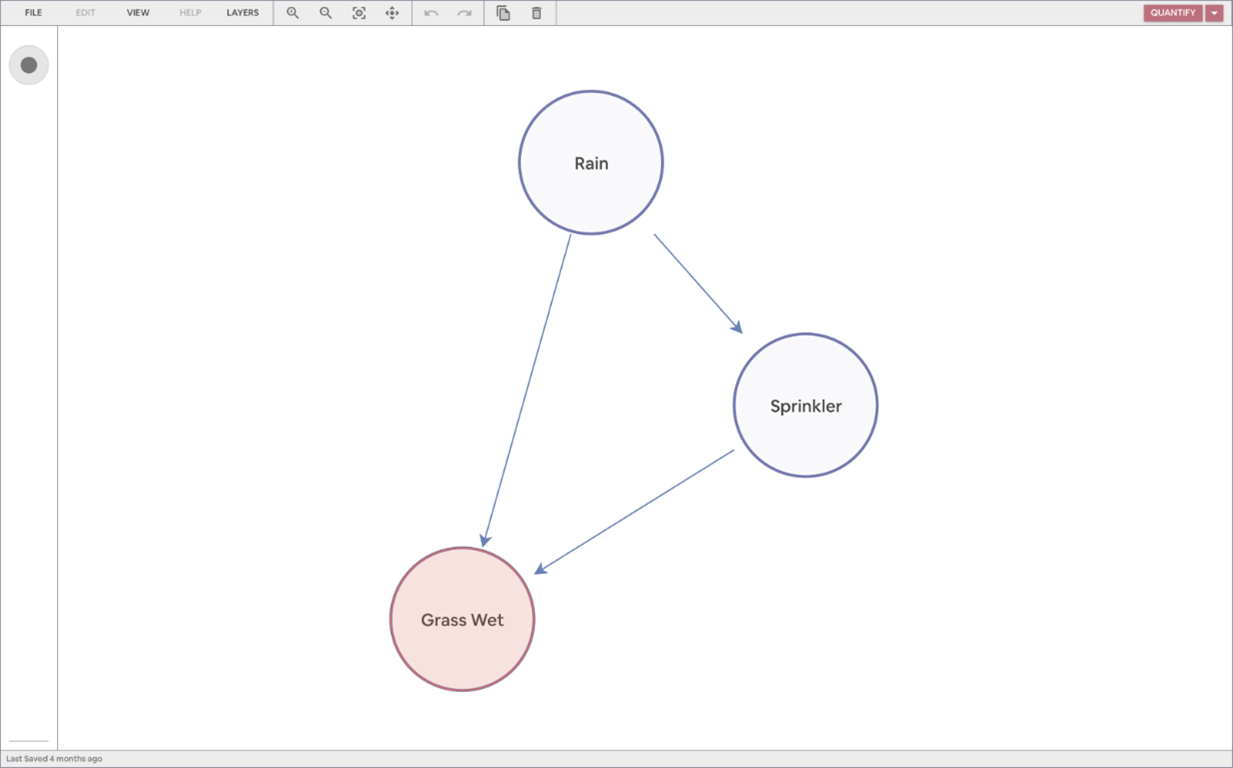
\includegraphics[width=\textwidth]{4_proposed_solution/web_app/figures/bn.png}
  \caption{Bayesian network editor.}
  \label{fig:bn_editor}
\end{figure}

OpenPRA currently uses \acrshort{hcla} as its default analyzer but is transitioning to the scram engine, with plans to phase out \acrfull{hcla} due to its proprietary license. To support advanced users, developers, and industry partners, OpenPRA offers \acrfull{api}s, tooling, and integration guides for adding custom or third‑party engines enabling on‑premise deployments and accommodating specific licensing requirements. Users can choose among multiple quantification engines when solving risk models. The front‑end provides interfaces for the following solvers:

\begin{itemize}
  \item \textbf{scram:} A command‑line tool for quantifying models specified in the OpenPSA \acrshort{mef} \acrshort{xml} schema. It implements \acrshort{bdd} for exact probability calculations, \acrshort{mocus}, along with \acrshort{mcub} and \acrshort{rea}, and \acrshort{zdd}, and supports uncertainty analysis via Monte Carlo simulation, importance analysis, and common cause failure groups (CCFGs).
  \item \textbf{XFTA:} Provides advanced fault tree quantification algorithms including cut‑set enumeration, \acrshort{mcs} generation, and importance analysis and implements \acrshort{bdd}, \acrshort{mocus}, and \acrshort{zdd} in version 2 and above.
  \item \textbf{Saphsolve:} The proprietary engine behind \acrshort{saphire}, supporting event tree analysis, fault tree analysis, and uncertainty analysis through its suite of quantification algorithms.
  \item \textbf{PRAQuant:} The default, proprietary fault tree quantification engine in Phoenix Architect, optimized for detailed fault tree analysis.
  \item \textbf{FTREX:} An optional, proprietary Phoenix Architect engine for fault tree quantification that offers additional algorithm choices.
  \item \textbf{Custom quantification engines:} Enables users to develop and integrate custom engines written in C++, Python, Java, etc. via OpenPRA’s \acrfull{api}s, allowing tailored quantification workflows.
\end{itemize}

\begin{figure}[h!]
  \centering
  \begin{subfigure}[b]{0.49\textwidth}
    \centering
    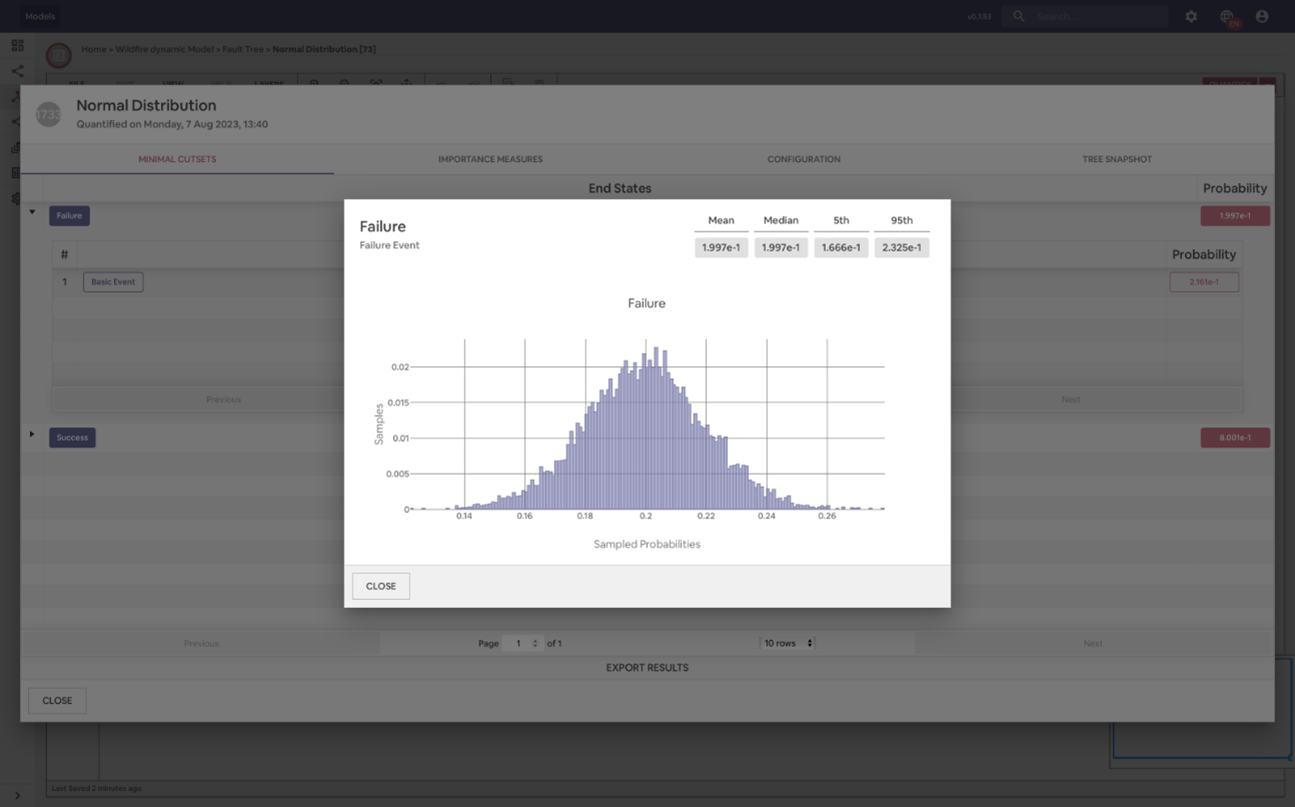
\includegraphics[width=\textwidth]{4_proposed_solution/web_app/figures/cutsets_uncertainty.png}
    \caption{}
  \end{subfigure}
  \begin{subfigure}[b]{0.49\textwidth}
    \centering
    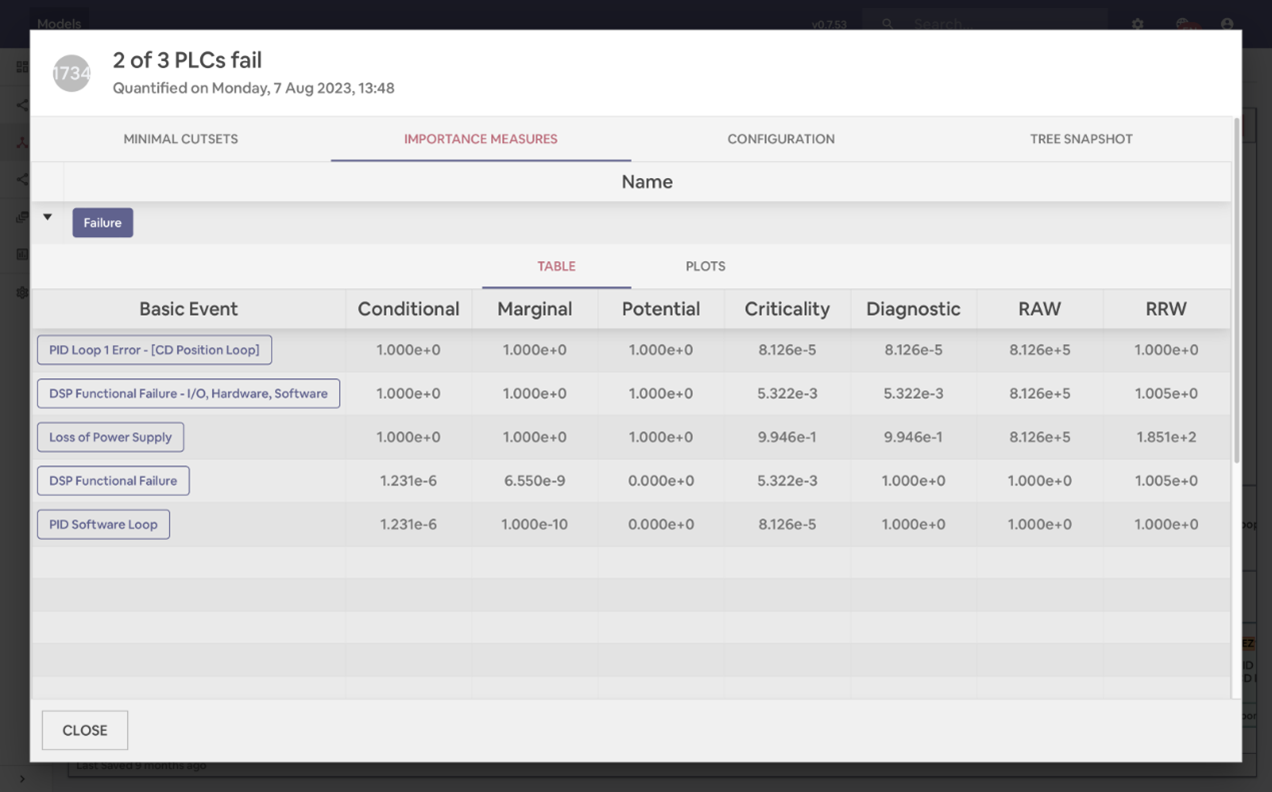
\includegraphics[width=\textwidth]{4_proposed_solution/web_app/figures/importance.png}
    \caption{}
  \end{subfigure}
  \begin{subfigure}[b]{0.49\textwidth}
    \centering
    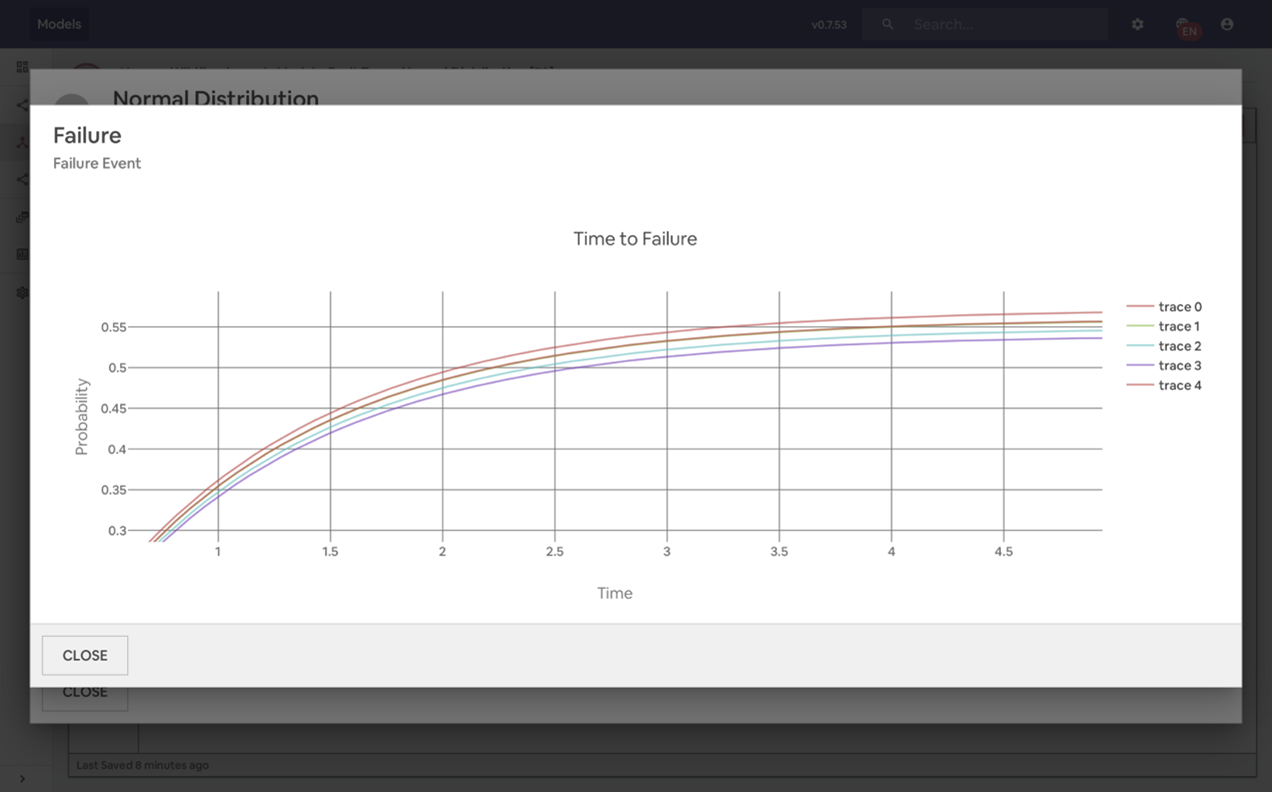
\includegraphics[width=\textwidth]{4_proposed_solution/web_app/figures/ttf.png}
    \caption{}
  \end{subfigure}
  \caption{(a) Cut sets, uncertainty using Monte Carlo sampling, (b) Importance measures calculation, (c) Time to failure cumulative distribution function with uncertainty quantification.}
  \label{fig:quantification_results}
\end{figure}

\section{Testing and Documentation}
\label{sec:testing_and_documentation}

\subsection{Source-code Testing}

The OpenPRA web application employs an automated and comprehensive testing strategy to ensure the correctness and reliability of its codebase. Static type checking is enforced throughout the front-end, backend, and distributed system components, all of which are implemented in TypeScript, as well as in the scram-node engine, which is written in C++. The use of statically typed languages enables the detection of type-related errors at compile time, thereby reducing the likelihood of runtime failures. In addition to compile-time checks, runtime type validation is performed using a dedicated library, which provides an additional layer of security by preventing invalid or malicious data from propagating through the system.

A continuous integration and deployment (CI/CD) pipeline is established to automate the quality assurance process. Each time a developer pushes code to the remote repository, an automated job is triggered. This job executes a series of static and dynamic tests, including static analysis, code linting, unit tests, and end-to-end tests. The pipeline ensures that the codebase builds correctly and that all tests pass before any changes are merged or deployed. In parallel, the continuous deployment process automatically deploys the application to the target infrastructure, ensuring that the latest validated version is available for use.

Testing in OpenPRA is designed to verify not only the correctness of individual components but also the integrity of their interactions and the stability of the application under evolving requirements and heavy usage. The testing framework encompasses unit, functional, regression, end-to-end, and stress tests, each serving a distinct purpose in the software quality assurance process.

\subsubsection{Unit Testing}

Unit tests are implemented to validate the behavior of isolated components and functions. In the front-end, these tests target interactive elements such as buttons, menus, navigation bars, and text fields, ensuring that user interactions result in the correct manipulation of the Document Object Model (DOM). On the backend, unit tests focus on controller methods, verifying that input parameters and HTTP responses conform to expected behaviors. Within the distributed system, unit tests confirm that quantification jobs are correctly enqueued and managed. The Jest library is used extensively for unit testing in the TypeScript codebase, while the Boost library is employed for unit tests in the C++ scram-node engine.

\subsubsection{Functional Testing}

Functional tests are designed to assess the correct operation of larger application features and their integration. In the front-end, these tests cover workflows such as user registration, authentication, and the use of web editors for constructing fault trees, event trees, event sequence diagrams, and Bayesian networks. Functional testing also verifies that the front-end correctly issues API requests in response to user actions and that the backend services are properly coupled to controllers and can interact with the database and job broker. In the scram-node engine, functional tests ensure that input parameters are correctly propagated through subroutine calls and that error handling mechanisms are effective when processing invalid input data.

\subsubsection{Regression Testing}

Regression tests are employed to detect unintended side effects or defects introduced by code modifications. These tests are particularly important for features that are expected to remain stable across releases. For instance, regardless of changes to the graphical representation of models in the web editor, the generated models must always conform to the OpenPRA MEF standard when transmitted via API requests.

\subsubsection{End-to-End Testing}

End-to-end tests simulate complete user workflows, encompassing the entire application stack from the front-end to the backend and distributed system. These tests begin with user account creation, proceed through model construction and quantification, and include subsequent actions such as authentication and model management. The backend is tested for its ability to process quantification requests, interact with the scram-node engine, and manage database operations. The distributed system is evaluated for its ability to coordinate job queuing, processing, and result delivery. Tools such as Playwright and SuperTest are used to automate these scenarios, launching the actual application components and executing predefined sequences of user actions to verify system wide correctness.

\subsubsection{Stress Testing}

Stress testing is conducted to evaluate the application's performance and stability under extreme load conditions. This involves simulating large numbers of concurrent users and repeated execution of end-to-end workflows to identify bottlenecks and establish baseline performance metrics. Stress tests measure parameters such as requests per second, average response time under load, and the maximum sustainable throughput of the backend, job queues, database, and quantification engine. These tests provide critical insights into the system's scalability and resilience.

\begin{landscape}
\begin{figure}
    \centering
    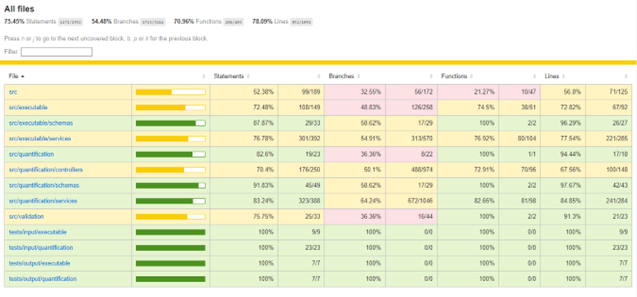
\includegraphics[width=1.3\textwidth]{4_proposed_solution/web_app/figures/test_coverage.png}
    \caption{Test coverage results for the distributed systems microservice.}
    \label{fig:test_coverage}
\end{figure}
\end{landscape}


\subsection{Automated Documentation Generation}

Documentation in OpenPRA is organized to serve both developers and end users. For developers, the documentation provides detailed descriptions of the core functionalities, interfaces, and methods of each component, facilitating quick onboarding and efficient maintenance. For users, the documentation offers guidance on interacting with the front-end, backend, distributed system, and engine as standalone packages, with a focus on API usage and integration.

\subsubsection{HTML-Formatted Documentation}

TSDoc comments are positioned above methods and inside classes across the front-end, back-end, and distributed system codebase to document input parameters, expected types, and output formats. In the C++ scram-node engine, Doxygen-style comments are used to document classes and methods. Inline comments are employed to clarify the use of third-party libraries and APIs, as well as to annotate test cases. Upon compilation, these comments are automatically converted into HTML documentation using tools such as TypeDoc, Compodoc, and Doxygen. The resulting HTML pages are accessible via dedicated URLs, providing a high-level overview of the codebase without requiring direct source code inspection.

% \begin{landscape}

% \end{landscape}

\subsubsection{Interactive API Documentation}

The backend and distributed system APIs are documented and made accessible through the Swagger UI, which adheres to the OpenAPI specification. Swagger automatically extracts endpoint definitions, supported operations, input and output schemas, and authentication requirements from the source code. It also allows for the inclusion of metadata such as titles, descriptions, tags, and licensing information. The interactive nature of Swagger enables users to explore and test API endpoints directly from the browser. Responses are returned in a standardized format, combining HTTP status codes with JSON payloads.

\begin{landscape}
\begin{figure}
    \centering
    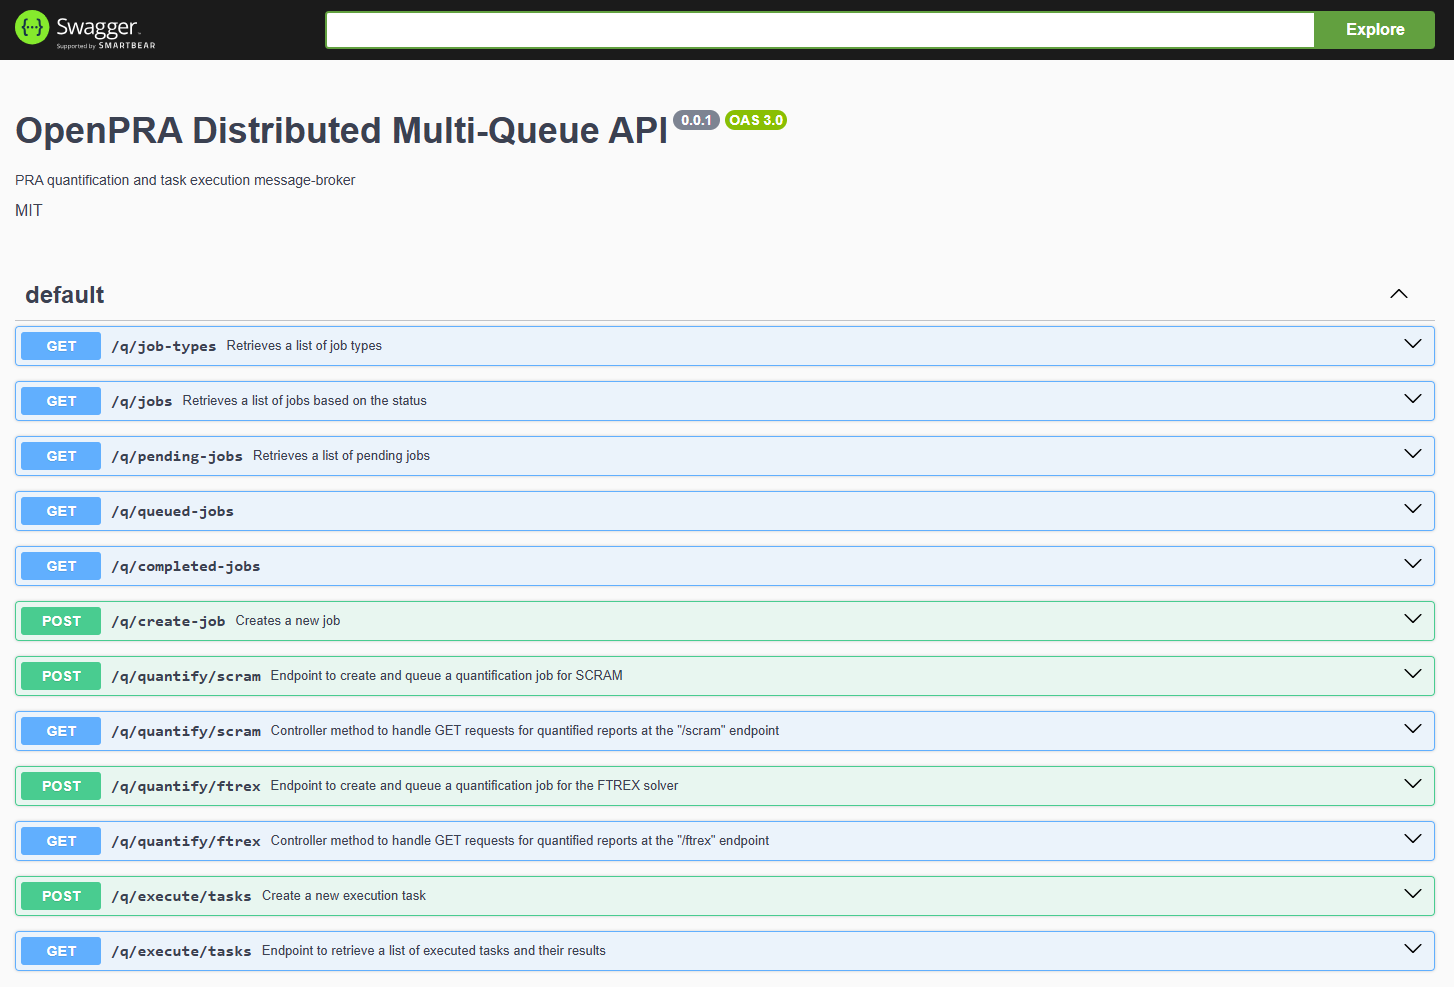
\includegraphics[width=1.3\textwidth]{4_proposed_solution/web_app/figures/swagger_doc.png}
    \caption{Interactive API documentation for the controller of distributed systems microservice.}
    \label{fig:swagger_doc}
\end{figure}
\end{landscape}

\subsection{Documentation for DevOps}

The OpenPRA project adopts DevOps best practices to streamline the software development lifecycle, emphasizing automation, continuous integration, and continuous deployment. Each standalone package, including the front-end, backend, distributed system, database, and scram-engine, is accompanied by a dedicated \texttt{readme.md} file containing detailed instructions for dependency installation, compilation, package execution, testing, and code formatting. Docker files are provided to automate environment setup and deployment, with comprehensive documentation on containerization workflows. These resources ensure that both developers and users have access to the necessary tools and guidance for effective development, testing, and maintenance of the OpenPRA platform.
